\input{../../../template.ltx}

\usepackage{graphicx}
\usepackage{bytefield}

% for aligning the letters in the bytefield
\newcommand{\baselinecenterit}[1]{%
  \centering
  \raisebox{0pt}[\heightof{W}][0pt]{\itshape #1}%
}

\begin{document}
\sloppy
\osuetitle{1}

\section*{Aufgabenstellung B -- Battleship}\label{sec:aufgabenstellung}
Implementieren Sie einen Client und einen Server, die mittels TCP/IP
miteinander kommunizieren. Dabei sollen der Client und der Server miteinander
``Battleship'' (deu.: ``Schiffe versenken'') spielen.

In diesem Spiel werden Schiffe auf einem Raster von 10x10 Kästchen platziert.
Die Schiffe haben unterschiedliche Längen und nehmen daher unterschiedlich viele Kästchen ein.
Schiffe dürfen nur horizontal oder vertikal platziert werden.
Die Position der Schiffe wird vor dem Gegenspieler geheim gehalten,
dessen Aufgabe es ist, die Schiffe zu versenken.
Dafür kann der Gegenspieler in jedem Spielzug einen Schuss auf ein Kästchen abfeuern.
Wurden alle Kästchen auf denen sich ein Schiff befindet getroffen, dann ist dieses Schiff versenkt.

Üblicherweise haben bei ``Battleship'' beide Spieler Schiffe und versuchen jeweils die des Gegners
zu versenken. In dieser Aufgabe wird eine reduzierte Version gespielt,
in der nur der Server Schiffe besitzt und der Client versucht diese zu versenken.
\emph{Beachten Sie, dass der Client vollautomatisch agieren soll}. Daher
ist die Implementierung einer Spielstrategie ebenfalls Teil der Aufgabe
(siehe Abschnitt~\nameref{sec:grading}).

In dieser Variante des Spiels gibt es folgende Schiffe:

{\centering
\begin{tabular}{ | l | l | l | }
\hline
Bezeichnung    & Anzahl & Länge \\
\hline
Schlachtschiff & 1 & 4 \\
Kreuzer        & 3 & 3 \\
Zerstörer      & 2 & 2 \\
\hline
\end{tabular}\par
}

Die Position der Schiffe wird dem Server durch Argumente auf der Kommandozeile
übergeben. Die Anordnung der Schiffe könnte zum Beispiel folgendermaßen aussehen:

{\centering
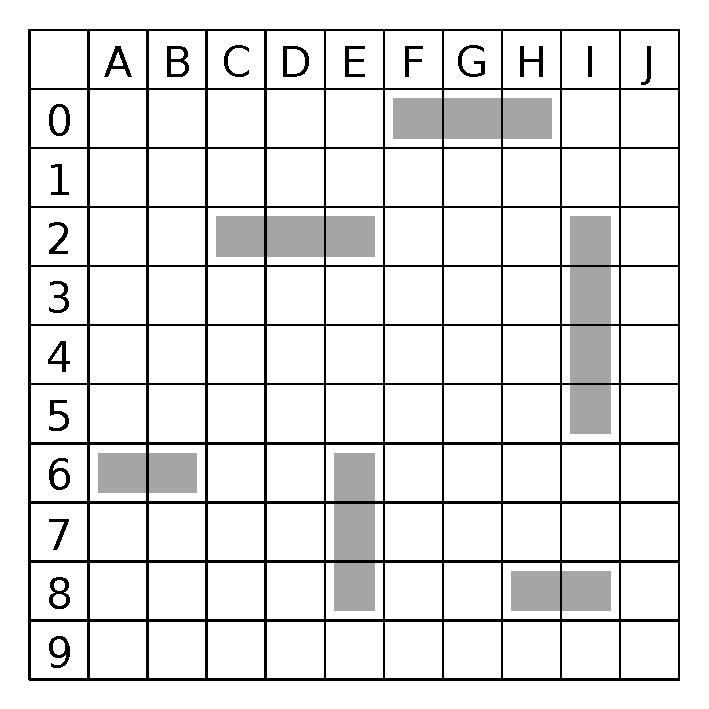
\includegraphics[scale=0.55]{map.pdf} \par
}

Nachdem eine Verbindung zwischen dem Client und dem Server hergestellt wurde,
wird sofort mit dem Spiel begonnen.
Der Client sendet die Koordinaten, auf die sein Schuss gerichtet ist
und der Server teilt ihm mit, ob er damit ein Schiff getroffen hat,
oder ob der Schuss ins Leere ging.
Im oben abgebildeten Spielfeld würde beispielsweise ein Schuss auf \textbf{A4} ins Leere gehen,
ein Schuss auf \textbf{D2} wäre ein Treffer.

Das Spiel endet, wenn der Client alle Schiffe versenkt hat, der Server einen
Protokollfehler meldet, oder die maximale Anzahl an Runden (\textbf{80})
erreicht wurde.

\subsection*{Implementierungshinweise}
\label{sec:implhints}

\begin{center}
\fbox{\parbox{0.95\linewidth}{
\textbf{Wichtig:} Beachten Sie, dass der wesentliche Teil in diesem Beispiel
die korrekte Implementierung der Kommunikation zwischen Client und Server ist.
Achten Sie auch darauf, dass Ihre Programme immer die richtigen Rückgabewerte verwenden!
}}
\end{center}

\paragraph{Server:}
Teile des Servers sind bereits vorgegeben. Bitte verwenden Sie dieses Template
und erweitern Sie es entsprechend.  Dem Server kann als Option der Port
übergeben werden, auf dem er für die Clients erreichbar sein soll.
Außerdem werden dem Server 6 Argumente übergeben, die die Positionen der 6 Schiffe angeben.
Jedes dieser Argumente hat Länge \textbf{4} und besteht aus den Koordinaten für Bug und Heck des Schiffes.
So beschreibt zum Beispiel der String ``\verb|C2E2|''
ein Schiff, welches die Kästchen \textbf{C2}, \textbf{D2} und \textbf{E2} einnimmt.

Der Server soll auf eingehende Verbindungen warten. Sobald eine Verbindung
akzeptiert wurde, beginnt ein neues Spiel, und der Server antwortet bis zum
Ende des Spiels auf die Anfragen des Clients.
Sobald der Server eine Anfrage erhält, soll er zunächst die Korrektheit des Paritätsbit in der Nachricht des Clients
überprüfen (siehe Abschnitt~\nameref{sec:prot}).
Sollte dieses falsch sein, antwortet der Server sofort mit dem entsprechenden Fehler-Status,
ohne den Rest der Nachricht zu verarbeiten.
Anschließend prüft der Server, ob die vom Client übermittelte Koordinate gültig ist
und informiert den Client darüber, ob er mit seinem Schuss ein Schiff getroffen hat.
Das Spiel endet sobald der Client alle Schiffe versenkt hat
oder wenn am Ende der 80.\ Runde noch immer Schiffe übrig sind.
Am Ende des Spiels soll die Verbindung geschlossen und das Programm beendet werden
(Rückgabewerte siehe weiter unten).

%Am Ende des Spiels wird entweder eine Fehlermeldung,
%oder die Anzahl der Spielrunden und die Anzahl versenkter Schiffe ausgegeben,
%und das Serverprogramm wird mit einem entsprechenden Rückgabewert (siehe weiter
%unten) beendet.

\vspace{-10pt}
\begin{verbatim}
Server:
    SYNOPSIS
        server [-p PORT] SHIP1...
    EXAMPLE
        server -p 1280 C2E2 F0H0 B6A6 E8E6 I2I5 H8I8
\end{verbatim}

\paragraph{Client:}

Dem Client können beim Aufruf der Hostname und die Portnummer des Servers
übergeben werden, ansonsten wird der Hostname per default auf \emph{localhost}
und der Port auf 1280 gesetzt. Legen Sie zuerst einen
TCP/IP-Socket an. Stellen Sie dann die zum Hostnamen des Servers zugehörige
IP-Adresse fest, und verbinden Sie sich mit dem Server. Danach wird sofort mit
dem Spiel begonnen, und der Client übermittelt wiederholt die Koordinaten,
die durch seinen Schuss getroffen werden, bis der Server kommuniziert,
dass alle Schiffe versenkt wurden, die maximale Rundenanzahl erreicht wurde
oder einen Fehler übermittelt.
%Am Ende des Spiels wird entweder eine Erfolgsmeldung (falls das Spiel gewonnen wurde)
%oder der zuletzt übermittelte Fehler ausgegeben.
Danach soll der Socket geschlossen und das
Programm beendet werden (Rückgabewert siehe nächster Absatz).

\vspace{-10pt}
\begin{verbatim}
Client:
    SYNOPSIS
        client [-h HOSTNAME] [-p PORT]
    EXAMPLE
        client -h localhost -p 1280
\end{verbatim}

% Verbinden Sie den Socket mittels \emph{connect}. Senden Sie mittels \emph{write} die Anfragen an de Server, und empfangen Sie de Antwort des Servers mittels \emph{read} und schicken ihn mittels \emph{write} wieder zurück.
\paragraph{Fehlermeldungen und Rückgabewerte:}

Falls der Server in seiner Antwort einen Fehler anzeigt, sollen sowohl der Client als auch der Server terminieren.
Bei einem Paritätsfehler sollen beide Programme die Meldung ``Parity error'' ausgeben
und beide Programme mit dem Wert 2 beenden.
Wenn der Server meldet, dass der Client einen ungültige Koordinate übertragen hat,
geben Sie in beiden Programmen die Meldung ``Invalid coordinate'' aus und beenden Sie beide Programme mit dem Exit-Code 3.
Bei sonstigen Fehlern (z.B.\ ungültige Kommandozeilenargumente, Verbindungsfehler, \ldots)
soll eine informative Fehlermeldung ausgegeben und mit Rückgabewert
\osueconst{EXIT\_FAILURE} (1) terminiert werden. Alle Fehlermeldungen müssen auf
\osueglvar{stderr} ausgegeben und von einem Zeilenumbruch gefolgt werden.

Das Spiel endet regulär wenn der Client alle Schiffe versenkt hat oder die maximale Rundenanzahl erreicht wurde.
Gelingt es dem Client alle Schiffe zu versenken, so soll der Server die Anzahl gespielter Runden auf \osueglvar{stdout} ausgegeben und beide
Programme mit Rückgabewert 0 beendet werden.
Wenn es dem Client nicht gelingt in 80 Runden alle Schiffe zu versenken, dann sollen beide Programme die Meldung ``Game lost'' auf \osueglvar{stdout} ausgeben
und ebenfalls mit Rückgabewert 0 terminieren.

Sobald der Server eines der Signale \osueconst{SIGINT} oder
\osueconst{SIGTERM} empfängt, soll der Serversocket geschlossen und das
Programm mit Rückgabewert 0 beendet werden.

\subsection*{Protokoll}
\label{sec:prot}

\begin{center}
\fbox{\parbox{0.95\linewidth}{
\textbf{Wichtig:} Achten Sie darauf, dass Sie das Protokoll exakt so implementieren, wie nachfolgend beschrieben!
Die korrekte Implementierung des Protokolls wird beim Abgabegespräch überprüft, Abweichungen sind nicht zulässig.
Insbesondere wird dabei auch festgestellt, ob Ihre Programme korrekt auf Fehler reagieren,
also ob beispielsweise Ihr Server einen Paritätsfehler oder ungültige Koordinaten erkennt
und ob Ihr Client auf Fehlermeldungen korrekt reagiert.
Überlegen Sie sich geeignete Tests, um die Korrektheit Ihrer Implementierung sicherzustellen!
}}
\end{center}

\emph{Server} und \emph{Client} kommunizieren in Runden wie nachfolgend
gezeigt. Der Client übermittelt pro Runde genau zwei Bytes,
der Server antwortet mit genau einem Byte.

\subsubsection*{Client}
Der \emph{Client} schickt an den Server Nachrichten im folgenden Format:

{\centering
\begin{bytefield}[boxformatting={\baselinecenterit},bitwidth=2.2em,endianness=big]{16}
   \bitheader{0-15} \\
   \bitbox{1}{p} & \bitbox{3}{unused} & \bitbox{6}{x} & \bitbox{6}{y}
\end{bytefield} \par
}

Die Werte \verb|x| und \verb|y| entsprechen dabei den Koordinaten des Kästchens,
welches durch den Schuss des Client getroffen wird,
wobei \verb|x| der Spalten-Index (Spalte \textbf{A}: Index 0, \textbf{B}: 1, \textbf{C}: 2, \ldots)
und \verb|y| der Zeilen-Index des Kästchen ist.
Beispielsweise entspricht das Kästchen \textbf{B5}
den Indizes $\verb|x|=1$ und $\verb|y|=5$.

Der Wert \verb|p| entspricht einem \emph{Parity Bit}\footnote{\url{https://en.wikipedia.org/wiki/Parity_bit}}
über die restlichen Bits der Nachricht (Bit~0 bis Bit~14).
Um dieses zu Berechnen, werden die einzelnen Bits mit
einer \emph{xor}-Operation verknüpft.
Wir verwenden \emph{even parity}, so dass die gesamte Nachricht immer aus einer geraden Anzahl an 1-Bits besteht.

Das Feld \verb|unused| wird nicht verwendet, die entsprechenden Bits sollten auf 0 gesetzt werden.

Da die Nachricht aus mehr als einem Byte besteht, ist es wichtig die
Byte-Reihenfolge\footnote{\url{https://de.wikipedia.org/wiki/Byte-Reihenfolge}} zu beachten:
Der Client muss zuerst das Byte mit den niederwertigen Bits (Bit~0 bis Bit~7)
und anschließend das Byte mit den höherwertigen Bits (Bit~8 bis Bit~15) übertragen.

\subsubsection*{Server}

Der \emph{Server} empfängt die Nachricht des Clients und überprüft, ob durch den
Schuss eines seiner Schiffe getroffen wurde. Anschließend sendet der Server eine
Antwort im folgenden Format:

{\centering
\begin{bytefield}[boxformatting={\baselinecenterit},bitwidth=2.2em,endianness=big]{8}
   %\settowidth{\bitwidth}{~number white~}
   \bitheader{0-7} \\
   \bitbox{4}{unused} & \bitbox{2}{status} & \bitbox{2}{hit}
\end{bytefield} \par
}

\verb|hit| teilt dem Client mit, ob ein Schiff getroffen wurde und gibt auch Auskunft darüber,
ob dieses versenkt wurde. Das Feld kann folgenden Werte annehmen:

{\centering
\begin{tabular}{ | c | l | }
\hline
\verb|hit| & Bedeutung \\
\hline
0 & Nichts getroffen (der Schuss ging ins Leere) \\
1 & Ein Schiff wurde getroffen (aber nicht versenkt) \\
2 & Ein Schiff wurde getroffen und damit versenkt, aber es gibt noch weitere Schiffe \\
3 & Das letzte Schiff wurde versenkt (der Client gewinnt) \\
\hline
\end{tabular}\par
}

Das Feld \verb|status| informiert den Client über den Spielstatus und eventuelle Fehler,
die in seiner letzten Nachricht enthalten waren.
Falls \verb|status| einen Fehler anzeigt wird das Feld \verb|hit| ignoriert und die entsprechenden Bits sollten auf 0 gesetzt werden.
Folgende Werte können in \verb|status| enthalten sein:

{\centering
\begin{tabular}{ | c | l | }
\hline
\verb|status| & Bedeutung \\
\hline
%0 & Keine Fehler \\
0 & Spiel läuft \\
1 & Spiel beendet (Alle Schiffe versenkt oder maximale Rundenzahl erreicht) \\
2 & Fehler: Die letzte Nachricht enthielt ein ungültiges Parity Bit \\
3 & Fehler: Die letzte Nachricht enthielt eine ungültige Koordinate \\
%3 & Die maximale Anzahl an Spielzügen wurde erreicht (Spielende) \\
\hline
\end{tabular}\par
}

Das Feld \verb|unused| wird nicht verwendet, die entsprechenden Bits sollten auf 0 gesetzt werden.

\subsection*{Bewertung}
\label{sec:grading}
Um das Beispiel erfolgreich zu lösen, müssen sowohl die Implementierung des
Servers als auch des Clients korrekt funktionieren (siehe allgemeine
Beispielanforderungen) und folgenden Anforderungen genügen:

\paragraph{Server:}
%Teile des Servers sind bereits vorgegeben. Bitte verwenden Sie dieses Template
%und erweitern Sie es entsprechend.

Der Server muss nach dem Start die Argumente, die er von der Kommandozeile erhält, analysieren
und falls ungültige Optionen oder Argumente übergeben wurde mit einer \textbf{usage}-Meldung terminieren.
Dabei muss auch überprüft werden, ob die angegebenen Positionen der Schiffe gültig sind,
also ob die entsprechenden Kästchen sich auf der Karte befinden und ob die Schiffe horizontal oder vertikal ausgerichtet sind.
Anschließend muss der Server auf eine eingehende Verbindung warten.
Falls ein alternativer Port als Option übergeben wird, hat der Server auf Verbindungen an diesem Port zu warten,
ansonsten ist Port 1280 zu verwenden.

Sobald ein Client eine Verbindung zum Server hergestellt hat, beginnt das Spiel und der Server wartet auf Anfragen des Client.
Während des Spiels muss der Server mitverfolgen welche seiner Schiffe an welchen Stellen getroffen wurden
und den Client korrekt darüber informieren, wenn ein Schiff getroffen oder versenkt wurde
und wenn alle seine Schiffe versenkt wurden.
Falls der Client bei der Übermittlung ein falsches Paritätsbit oder ungültige Koordinaten sendet,
oder es ihm nicht gelingt in 80 Zügen alle Schiffe zu versenken,
hat der Server wie im Abschnitt~\nameref{sec:implhints} beschrieben darauf zu reagieren.

\paragraph{Client:}
Nach dem Start muss der Client die Argumente, die er von der Kommandozeile erhält, analysieren
und falls ungültige Optionen übergeben werden mit einer \textbf{usage}-Meldung terminieren.
Insbesondere dürfen die in Abschnitt~\nameref{sec:implhints} beschriebenen Optionen höchstens einmal
übergeben werden und es dürfen im Anschluss an die Optionen keine weiteren Argumente mehr folgen.
Anschließend muss der Client eine Verbindung zum Server unter dem angegebenen Hostnamen (oder \textbf{localhost}
falls keine Hostname übergeben wurde) und dem angegebenen Port (oder 1280 falls kein Port übergeben wurde)
herstellen.

Sobald der Client eine Verbindung zum Server hergestellt hat beginnt das Spiel
und der Client sendet seine erste Anfrage.
%und der Client muss jeweils innerhalb von einer Sekunde (auf
%dem Abgaberechner im TI-Labor) eine Anfrage an den Server generieren.
% Weiters muss jedes Spiel innerhalb von 35 Runden gewonnen werden.
Sendet der Server einen Fehlercode, so muss der Client sofort mit der
entsprechenden Fehlermeldung terminieren.

\paragraph{Bonuspunkte:} Für gute und ausgezeichnete Lösungen werden Bonuspunkte vergeben.
\textbf{Bonuspunkte werden nur vergeben, wenn der Client und der Server korrekt funktionieren.}

\begin{itemize}
    \item \textbf{Server:} Sie erhalten 2 Bonuspunkte wenn Ihr Server überprüft,
    ob die korrekte Anzahl an Schiffen mit einer bestimmten Länge übergeben wurde (wie in Abschnitt~\nameref{sec:aufgabenstellung} beschrieben),
    und ob zwischen den Schiffen jeweils mindestens ein Kästchen frei bleibt, also zwei Schiffe nie aneinander grenzen
    (auch nicht in diagonaler Richtung). Falls nicht, soll der Server mit einer \textbf{usage}-Meldung terminieren.
    \item \textbf{Client:} Zur Ermittlung der Bonuspunkte Ihres Client wird dieser mit dem vom Institut implementierten Server getestet
    und durchläuft dabei mehrere Test-Spiele. Die Tests bestehen ausschließlich aus gültigen Konfigurationen,
    also mit den in Abschnitt~\nameref{sec:aufgabenstellung} angegebenen Schiffen,
    wobei zwei Schiffe nie aneinander grenzen (auch nicht in diagonaler Richtung).
    Sie erhalten 2 Bonuspunkte, wenn Ihr Client jedes Spiel gewinnt.
    Außerdem können Sie bis zu 6 weitere Bonuspunkte erhalten,
    wenn Ihr Client jedes Spiel gewinnt und dafür durchschnittlich besonders wenig Züge benötigt:

    \vspace{3pt}
    {\centering
    \begin{tabular}{| c | c | c | c |}
    \hline
    Durchschnittliche Anzahl an Zügen & $<70$ & $<55$ & $<40$ \\
    \hline
    Zusätzliche Bonuspunkte & 2 & 4 & 6 \\
    \hline
    \end{tabular} \par
    }
\end{itemize}

\subsection*{Testfälle}
\label{sec:testcases}

Die folgenden Testfälle können Sie als Hilfestellung verwenden, um Ihre Implementierung zu testen.
Außerdem sollen Sie Ihnen als Beispiel dienen für die Ausgaben, die von Ihren Programmen erwartet werden.

\subsubsection*{Fehlermeldungen beim Programmaufruf:}
\vspace{-10pt}
Server:
\vspace{-10pt}
\begin{verbatim}
$ ./server -x G1I1 C5E5 A7B7 G6G8 I9J9 B0E0
./server: invalid option -- 'x'
usage: ./server [-p PORT] SHIP1...
$ ./server G1I1 C5E5 A7B77 G6G8 I9J9 B0E0
[./server] ERROR: wrong syntax for ship coordinates: A7B77
$ ./server G1I1 C5E5 A7Z7 G6G8 I9J9 B0E0
[./server] ERROR: coordinates outside of map: A7Z7
$ ./server G1I1 C5E5 A7B9 G6G8 I9J9 B0E0
[./server] ERROR: ships must be aligned either horizontally or vertically: A7B9
\end{verbatim}

Client:
\vspace{-10pt}
\begin{verbatim}
$ ./client -x
./client: invalid option -- 'x'
usage: ./client [-h HOSTNAME] [-p PORT]
$ ./client arg
usage: ./client [-h HOSTNAME] [-p PORT]
\end{verbatim}

\subsubsection*{Fehlermeldungen während des Spieles:}
\vspace{-10pt}
Paritätsfehler:
\vspace{-10pt}
\begin{verbatim}
$ ./server G1I1 C5E5 A7B7 G6G8 I9J9 B0E0 & sleep 1 && ./client
[./server] ERROR: parity error
[./client] ERROR: parity error
\end{verbatim}

Ungültige Koordinate:
\vspace{-10pt}
\begin{verbatim}
$ ./server G1I1 C5E5 A7B7 G6G8 I9J9 B0E0 & sleep 1 && ./client
[./server] ERROR: invalid coordinate
[./client] ERROR: invalid coordinate
\end{verbatim}

Client verliert:
\vspace{-10pt}
\begin{verbatim}
$ ./server G1I1 C5E5 A7B7 G6G8 I9J9 B0E0 & sleep 1 && ./client
[./server] game lost
[./client] game lost
\end{verbatim}

Client gewinnt:
\vspace{-10pt}
\begin{verbatim}
$ ./server G1I1 C5E5 A7B7 G6G8 I9J9 B0E0 & sleep 1 && ./client
[./server] client wins in 77 rounds
[./client] I win :)
\end{verbatim}

\osueguidelinesone

\end{document}

